\documentclass{beamer}

\usepackage[utf8]{inputenc}
\usepackage[english]{babel}
\usepackage{graphicx}
\usepackage[backend=bibtex, style=verbose-ibid, bibstyle=ieee]{biblatex}


\graphicspath{ {./images/} }
\addbibresource{cosc428.bib}

%Information to be included in the title page:
\title{Dice Detection and Classification}
\author{J. P. Sheehan}
\institute{University of Canterbury}
\date{\today}

\usetheme{Madrid}

% set smaller footnote font size
\setbeamerfont{footnote}{size=\tiny}

% remove beamer navigation buttons
\setbeamertemplate{navigation symbols}{}

\begin{document}

\frame{\titlepage}

%%%%%%%%%%%%%%%%% Outline
% This is a brief outline/overview of the presentation

\begin{frame}
\frametitle{Presentation Outline}

\begin{enumerate}
	\item Introduction
	\item Background Research
	\item Method
	\item Conclusion
\end{enumerate}

\end{frame}



%%%%%%%%%%%%%%%%% Introduction
% Goal/problem statement (what is your goal/what problem are you solving)

\begin{frame}
\frametitle{Introduction}

\begin{itemize}
	\item Dice value identification is important in industries such as gaming, and disability assistance.
	\item Most people have access to a device that can capture imagery and process it in realtime.
	\item This is a good fit for computer vision and machine learning.
\end{itemize}

\vspace{\baselineskip}

\begin{figure}
	\centering
	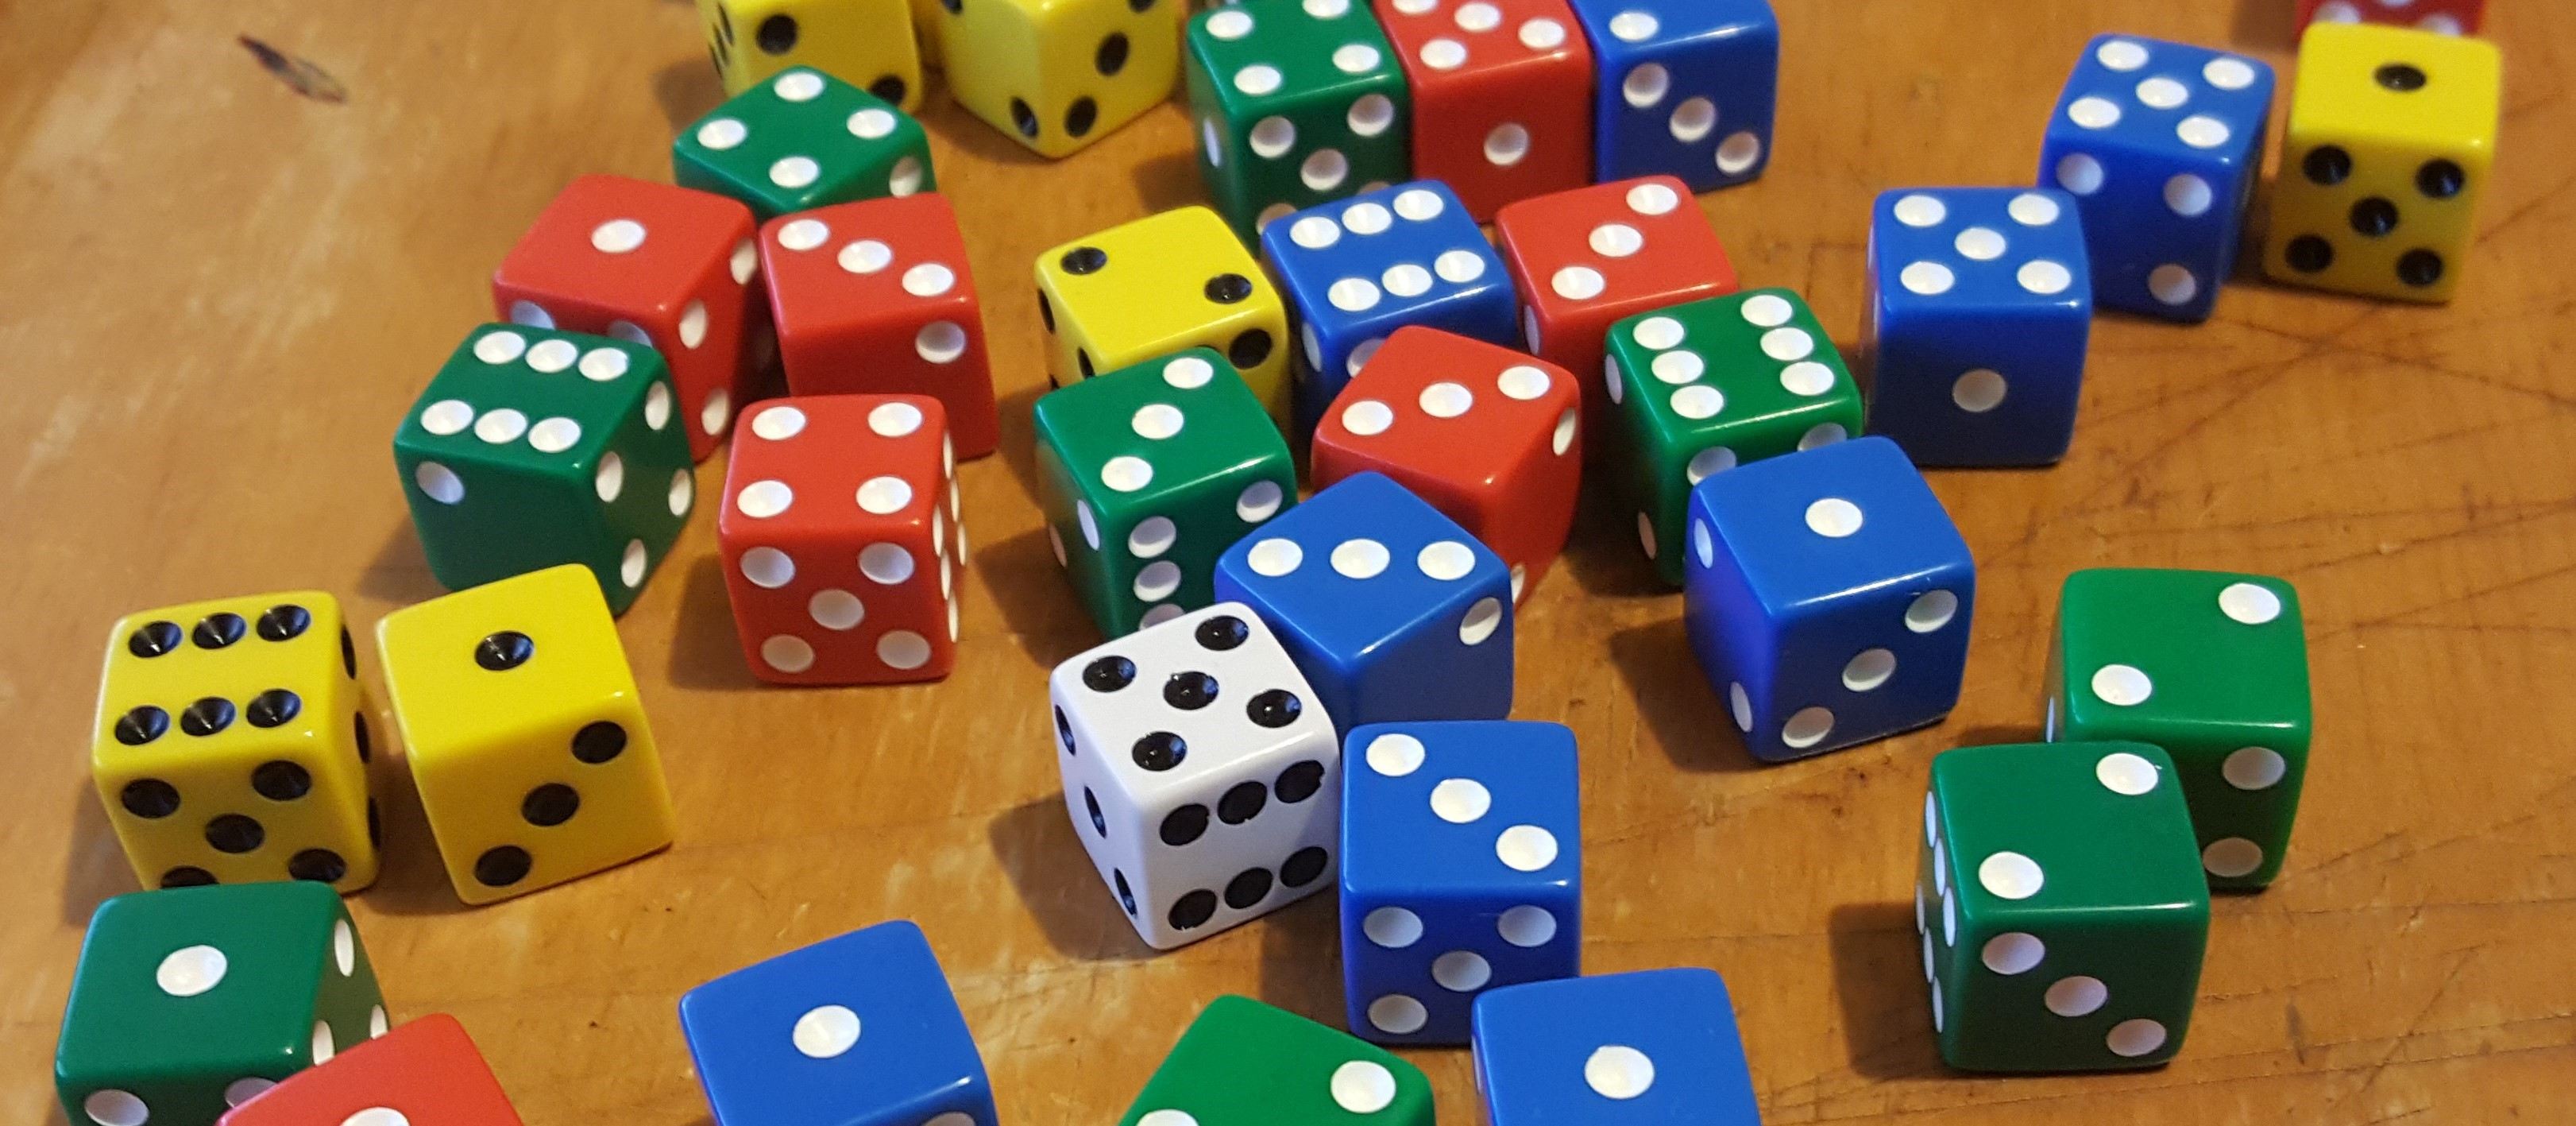
\includegraphics[width=0.6\textwidth]{intro}
\end{figure}
	
\end{frame}



%%%%%%%%%%%%%%%%% Background
% (focused specifically on concepts/papers related directly to your work – not too general)
% - Cite publications critically (be critical of prior research => mention limits/constraints/etc) – references appear as footnotes on background slides
% - Equations (you may be able to find many of these in other papers/text books.
% - Diagrams (you may be able to find many of these in other papers/text books.
% - Images (you may be able to find many of these in other papers/text books.
% - References as footnotes on as many relevant slides as possible
% - Summarise limitations of prior research (the entire reason for doing this paper and also shows that you can read critically)

% https://sci-hub.tw/https://doi.org/10.1117/12.205506
% B. A. B. Correia, J.A. Silva, F. D. Carvalho, R. Guilherme, F. C. Rodrigues, and A. M. de Silva Ferreira ``Automated Detection and Classification of Dice'', 
\begin{frame}
\frametitle{Automated Detection and Classification of Dice (1995)\footcite{Correia1995}}

The ``SORTE'' system was commissioned by the Portuguese Gaming Inspection Authorities for use in casinos.

\vspace{\baselineskip}

\begin{columns}

\column{0.5\textwidth}

Limitations:
\begin{itemize}
	\item Designed for a specific kind of die and surface.
	\item Requires a birds-eye view.
	\item Requires a careful lighting setup.
\end{itemize}

\column{0.5\textwidth}

\begin{figure}
	\centering
	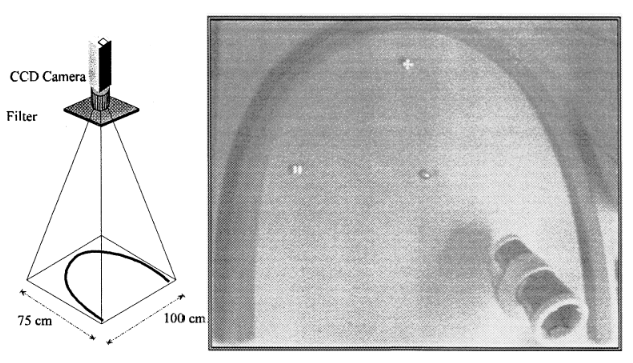
\includegraphics[width=\textwidth]{prior_1a}
\end{figure}

\end{columns}
	
\end{frame}

% https://sci-hub.tw/https://ieeexplore.ieee.org/document/854173
\begin{frame}
\frametitle{Computer Vision Based Reliability Control for Electromechanical Dice Gambling Machine (2000)\footcite{Lapanjaa}}
	
This system was designed to detect dice rolls from within an electronic gaming machine.
Under controlled conditions, this method has a 100\% success rate.
	
\vspace{\baselineskip}

\begin{columns}

\column{0.5\textwidth}

Limitations:
\begin{itemize}
	\item Requires fixed die size.
	\item Requires fixed camera distance.
	\item Uses template matching for identification.
\end{itemize}

\column{0.5\textwidth}

\begin{figure}
	\centering
	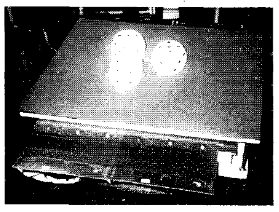
\includegraphics[width=0.8\textwidth]{prior_2a}
\end{figure}

\end{columns}

\end{frame}

% https://www.ncbi.nlm.nih.gov/pmc/articles/PMC3927534/
\begin{frame}
\frametitle{An Auto-Recognizing System for Dice Games Using a Modified Unsupervised Grey Clustering Algorithm (2008)\footcite{Huang2008}}

This algorithm uses a modified unsupervised gray clustering algorithm to determine the value of each die.

\vspace{\baselineskip}

\begin{columns}

\column{0.5\textwidth}

Limitations:
\begin{itemize}
	\item Requires birds-eye view.
	\item Requires number of dice to be known in advance.
	\item Requires low noise background.
\end{itemize}

\column{0.5\textwidth}

\begin{figure}
	\centering
	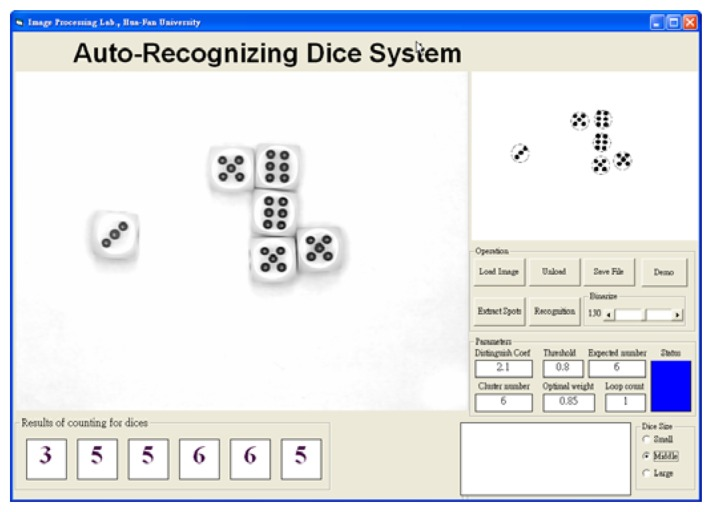
\includegraphics[width=0.9\textwidth]{prior_3a}
\end{figure}

\end{columns}
	
\end{frame}

% https://pdfs.semanticscholar.org/e5ce/5bd436211c8d7e168c03fae71b11f0648921.pdf
\begin{frame}
\frametitle{Image Identification Scheme for Dice Game (2009)\footcite{Chung2009}}

This algorithm uses image feature detection and the least distance criterion to detect die values.

\vspace{\baselineskip}

\begin{columns}

\column{0.5\textwidth}

Limitations:
\begin{itemize}
	\item Requires birds-eye view.
	\item Requires specific die colors and contrast with background.
	\item Only tested with four dice.
\end{itemize}

\column{0.5\textwidth}

\begin{figure}
	\centering
	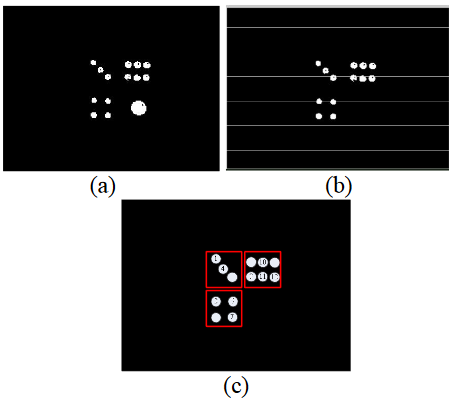
\includegraphics[width=0.8\textwidth]{prior_4a}
\end{figure}

\end{columns}
	
\end{frame}



%%%%%%%%%%%%%%%%% Solution/Method
% - How your proposed solution overcomes the limitations of prior research (as just mentioned)
% - Equations (may be old equation with slight tweak)
% - Diagrams
% - Images

\begin{frame}
\frametitle{Method}

Instead of performing perfectly under specific conditions, like all prior research, my method works under all conditions with mediocrity!

\begin{itemize}
	\item Image capture
	\item Image pre-processing
	\begin{itemize}
		\item Grayscale
		\item Binary threshold
		\item Gaussian blur
	\end{itemize}
	\item Canny edge detection
	\item Contour area and shape rejection
	\item Die face processing
	\begin{itemize}
		\item Face isolation
		\item Face rotation and resize
		\item Convolutional neural network\footnote{CNN trained on 1200 images to 97\% accuracy.} for value classification
	\end{itemize}
\end{itemize}

\end{frame}



%%%%%%%%%%%%%%%%% Results
% - Must be quantified – i.e. numbers, not just images
% - Graphs and/or tables
% - Images (lots of images available in a subject like computer vision)
% - Limitations of your proposed solution (gives more credibility)

\begin{frame}
\frametitle{Results}

The detection method:
\begin{itemize}
	\item Is rotation invariant.
	\item Will reliably detect yellow and white dice.
	\item Is not likely to go rogue and take over the world.
\end{itemize}

\vspace{\baselineskip}

Limitations:
\begin{itemize}
	\item Very sensitive to lighting levels and surface features.
	\item More work needs to be done to filter out noise.
\end{itemize}

\begin{columns}

\column{0.3\textwidth}

\begin{figure}
	\centering
	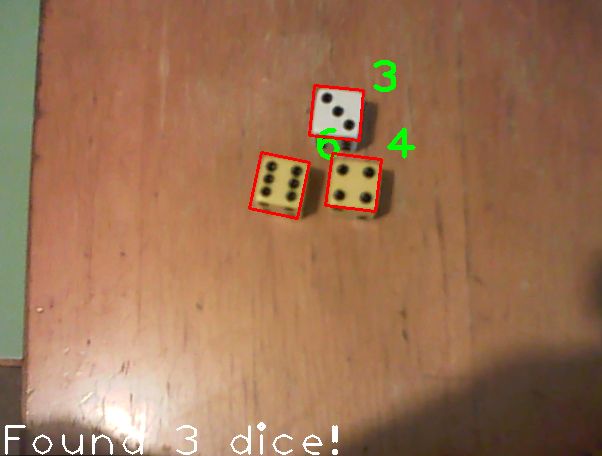
\includegraphics[width=\textwidth]{dice_1}
\end{figure}

\column{0.3\textwidth}

\begin{figure}
	\centering
	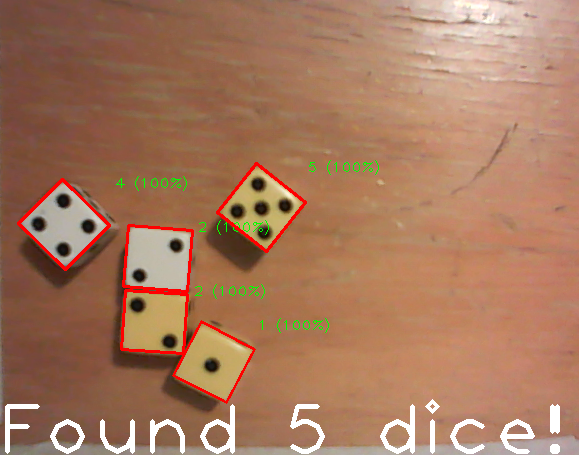
\includegraphics[width=\textwidth]{dice_2}
\end{figure}

\end{columns}
	
\end{frame}


%%%%%%%%%%%%%%%%% Conclusion
% - Results (very brief i.e. one sentence summing up results)
% - How your proposed solution compares with prior research (quantify and cite the prior research you are comparing with)
% - Limitations of your research (very brief)
% - Future research to overcome these limitations

\begin{frame}
\frametitle{Conclusion}

A dice detection method was designed using basic image processing and feature detection techniques.
A convolutional neural network was used to classify each die face with 97\% accuracy.

\vspace{\baselineskip}

Unlike prior research, the proposed solution works (somewhat) under a range of operating conditions.

\vspace{\baselineskip}

In future, more work needs to be done to remove noise and lighting artifacts during image pre-processing and to support detection of dark-coloured dice.
	
\end{frame}

\end{document}